This chapter describes the process of workload generation\index{Load generation} in detail. 
In order to build the model(s) proposed in Chapter~\ref{chap:thesis-arescue},
we adopt an empirical approach based on micro-benchmark profiling on the virtual
machines. For this, we intended to generate various types of loads 
(CPU, disk, intra-PM and inter-PM network loads) at different levels 
and measure the resultant CPU usage. There are quite a few tools 
available off-the-shelf for load generation. However, in many cases, these tools were
insufficient for our purposes. In this chapter, we describe the existing 
tools and their insufficiency, and also present the design of our
custom micro-benchmarks.

\section{Toolkit requirements}
The prime requirements of our workload generation step were as follows,
\begin{enumerate}
  \item We should be able to generate
load on various resources (CPU, network and disk) at variable rates, i.e., we need to exercise
progressively increasing (or decreasing) levels of activity within a range. 
  \item To create more realistic scenarios, we also need to generate workloads in combination, i.e.
load on multiple resources simultaneously
  \item Any load level chosen should generate a fixed
load, unless resource constrained by another parallelly executing workload, i.e., the interference
should only happen if the resource capacity is saturated, and not for any other reason.
\end{enumerate}

The load generation, logging and log transfer are to be automated via a script on a central
\textit{controller} machine in our setup. The script should ssh to specified VMs and PMs,
and start off load, start off logging, and later stop logging, stop load, and collect logs
into a specified central repository. To enable automatic ssh without prompting for manual
password input each time, 
need to perform secure ssh key exchange between \textit{controller} machine and all others.


\section{Unsuitability of existing tools for our micro-benchmarking experiments}
Our
first recourse was to search for existing load generators. We were able to find a huge set of
such tools per load type, say CPU, network I/O and disk I/O. We also found a few tools that
could generate more than one of these different load types. However, we found all of these tools
unsuitable for our purpose due to various reasons, as cited below.

\subsection{Existing tools for network traffic}
For generating rate-specific network loads, we initially experimented with creating
UDP\nomenclature{UDP:}{User Datagram Protocol} workloads. 
For this, we explored tools like bwUDP and iperf~\cite{iperf}. 
However, we observed that the tools themselves were causing
high CPU utilization in the DomU. We viewed such extra CPU usage as unacceptable ``noise''.
Besides, UDP workloads were not representative of most applications\textemdash{}which would
likely use TCP connections for communication. 
We also tried httperf~\cite{httperf} to generate file uploads
and downloads. However, we observed that the network traffic generation tools had
high CPU overhead for their usage, which was against our requirements.

\subsection{Existing tools for disk load generation}
For disk load generation, we explored several tools including 
IOzone~\cite{iozone}, Iogen~\cite{iogen}, 
Rugg~\cite{rugg}, LMBench~\cite{lmbench} and Vdbench~\cite{vdbench}.
However, we found that tools like Iogen, IOzone, Rugg and LMBench are designed
to ``stress test'' the disk and measure the resulting saturated I/O performance.
In other words, these tools offer no rate control. Moreover, the
Vdbench tool is written in Java, and resulted in around 60\% CPU 
utilization, which was not
acceptable since we required to measure the 
CPU utilization resulting purely due to the disk load being
generated and not due to the workload generator overhead. 

There are other tools which we were
unable to use, like HP's Disk Bench (DB), which is available only as part of HP Developer \&
Solution Partner Program (DSPP), 
and fio~\cite{fio} whose documentation was not very adequate at the time.
Intel IOMeter~\cite{iometer} was a possible option for disk load generation, 
however it is a platform
specific tool and had no AMD support (at that time, our working setup had AMD machines).

\subsection{Existing tools for CPU load generation}
For generating CPU load, 
we checked out a few tools like Lookbusy~\cite{lookbusy}, Load~\cite{load}, and
Stress~\cite{stress}. Lookbusy attempts to keep the total 
CPU utilization at a particular level, by 
manipulating its own activity level according to any 
other CPU usage that maybe already being incurred
on the machine. 
For example, if we request Lookbusy to generate 60\% CPU load, 
and if there is some other workload already executing which uses 20\% CPU,
then Lookbusy generates only an additional 40\% CPU usage to bring
the total to 60\%.
This is contrary to our needs, since 
we need CPU load of a particular level to
be generated irrespective of any other CPU utilization that may 
be present. 

The Stress tool simply ``stress-tests'' the 
system on various resource axis, and was not of much use 
for rate-controlled micro-benchmarking.
The Load tool generated CPU using two threads\textemdash{}a controller 
thread and a worker thread.
The controller thread starts off the worker and goes to sleep 
for a certain interval $x$, and stops
the worker thread after waking up. After waiting for an interval 
of 100−$x$ time units, the controller thread
starts off the execution of the worker thread. Hence the 
expected CPU utilization caused by the worker thread = $x$/100 = $x$\%. 
However, this is true only if the Load program is the only process executing
on the machine, and the presence of any other program would 
be unnoticed by the controller
thread, hence potentially resulting in lower than $x$\% utilization. 
Such kind of inherent 
interference during load generation is unacceptable for our 
purposes, at least during combinational load generation.
\\
\\
Due to the above problems, we resolved to build a custom load 
generation tool, using simple system commands \& programs, like 
\texttt{dd} for disk loads, \texttt{wget} and/or TCP socket programming 
for network loads, and Fibonacci series computation programs for 
CPU load. Our language of choice was C. The program can take
inputs regarding different types of loads and can spawn multiple 
threads, one for each workload type. Next, we describe in more detail 
the steps adopted to create various types of workloads.

\section{Custom micro-benchmarks}
Due to the inadequacy of existing workload generation tools for micro-benchmarking, we 
designed and implemented a customized workload generation tool. Implemented in C language,
it spawns separate threads for each workload type and can be used to generate CPU load (C),
disk read load (R), disk write load (W), and network load (N). This tool can be executed on
any machine (physical or virtualized) on which load generation is required, with appropriate
input parameters regarding the load level for each requested workload type. Combinational loads
(i.e., combination of any or all among cpu, disk-read, disk-write, intra-PM and inter-PM
network traffic)
can be generated by specifying inputs for each workload type and multiple load generating
threads are spawned accordingly. 

As mentioned previously, our intention is to generate various levels of loads for each
workload type, and then generate profiles for them. However, accuracy of load generation is not
mandatory, in the sense that, if the load requested is 90\% CPU utilization, the load generation
tool should generate utilization approximately close to 90\%, although it need not be exact. 
Similarly, when asked to generate 50M bps network
load, the tool may generate some network load in the range of 45 to 55M bps. However, the load
level thus generated (and observed) should be deterministic for the requested load (i.e., it
should generate the same requested level each time), and this is sufficient for our cause.

\subsection{CPU micro-benchmark}
We generate CPU workload by first computing off-line, the
first $2,000,000$ Fibonacci numbers and noting 
the time $T$ taken, say $T = 10ms$. Multiple such
Fibonacci computation operations consecutively
form a string of Fibonacci operations.
Different levels of CPU utilization are attained
by varying the length of such Fibonacci operation strings (\textit{active time}) and
the length of sleep time between consecutive strings (\textit{sleep time}). To generate a
CPU load of $X\%$, $X$ consecutive strings of $2,000,000$ Fibonacci numbers are
computed % (string length = $X$)
and then the computation thread sleeps for 
($100-X) \times T$. 

The difference between our approach, and the approach in Load~\cite{load} tool
is that we use a single thread to compute and sleep in such a manner that the 
required load is generated, whereas the Load tool uses two threads\textemdash{}worker and controller, 
such that worker does computation and controller causes it to sleep or awaken. In
the worker/controller setup, if there are other CPU-intensive loads present, the
worker may not have gotten enough computation time but the controller will still
suspend it because it is unaware of the external interference. However, in 
our case, a single thread is responsible for the CPU load generation, and can
better keep track of its own activity periods.

\subsection{Disk read \& write micro-benchmark}
We generate disk read (or write) workload by reading 
(or writing) files of a specific size, continuously one after the other, for a period of time
$T$ (say, one minute). 
In order to vary the disk read access rates (in read load), we need to to
overflow the RAM in such a manner that every read fetches 
data directly from the disk instead of finding it in cache. To
ensure this, for every file size input (example, $x$ KB) for disk read, 
we pre-create a base file set
containing files of size $x$ KB, such that 
the total size of the dataset is equal to twice the RAM size.
Since the files are read in the same order each time, 
it is ensured that after a file is read from
disk once, the next read request to that same 
file will happen only after that file’s previously
fetched contents have been flushed out of the RAM and cache, 
thus ensuring that disk access occurs.

\subsection{Network micro-benchmark}
In the first version of the tool, 
network receive load at a VM was generated by having the load generation
tool invoke \texttt{wget} on a URL to fetch a 128 KB file. 
The receive rate (or bandwidth) was controlled
by varying the sleep between consecutive file fetches. 
Similarly, to create network transmit load
at the VM, another VM invokes \texttt{wget} targeted at a 
URL on this VM. In other words, to create network
transmission load at VM1, \texttt{wget} requests are
generated at VM2 directed at VM1, which causes
VM1 to respond by transmitting the requested file. 
	
In the second version of the tool, we changed 
the network load generation functionality such that
the segment size of network transmission also could be varied. 
Specifically, instead of using 128 KB fixed
size files only, we generated various levels of 
network traffic between a pair of VMs by using
a TCP-based custom application that sends 
strings of bytes on a
TCP socket with different periodicity\textemdash{}the 
length of the byte string (referred to as segment size\index{segment size})
can also be varied to generate different levels of network traffic.
We assume the maximum available capacity to be $100Mbps$ and vary the load on each VM by steps
of $10Mbps$, from $10$ to $90 Mbps$. 
To generate various levels of network traffic, we varied
the transmission interval as well as the segment size of transmission.

\subsection{Mixed workloads}
In the above benchmarks, we have generated workloads that utilize one 
resource axis at a time. However, most applications would use more than
one resource for their execution.
Our load generation tool has a multi-threaded implementation, such that a thread 
can be spawned for each type of load (CPU, network or disk) to be generated.
Thus, combination workloads can be generated by spawning multiple threads, one 
for each load type and level. 
%However, it is not possible to cover
%the entire space of combinational workloads exhaustively, we randomly 
%select a representative batch of mixed workloads and execute them in 
%both dispersed and colocated cases in our benchmarking phase.

\section{Micro-benchmark workload intensities}
For our profiling step, we use a generic client-server setup (described earlier 
in Section~\ref{sec:arescue-setup}), wherein a client (the controller 
machine) remotely connects to the servers (each PM or Dom0, 
and VM or DomU) where workload is to be generated. The workload 
generation tool resides on each such logical ``server'' and complies 
with the load generation requests received from the logical ``client'' machine.

For CPU micro-benchmarking, we split the CPU load into nine different intensities ranging
from 10\% to 90\%. At each of the two VMs, we vary the CPU load from 10\% to 90\%, thus
resulting in 9 $\times$ 9 = 81 CPU workload combinations, as input for the modeling process. For
network loads, we assume the maximum available capacity to be 100 Mbps and vary the load on
each VM by steps of 10 Mbps, from 10 to 90 Mbps. For disk read and write micro-benchmarking,
we vary the file size from 4KB to 8MB, in powers of 2. 

In order to train the model on some realistic data, we also needed combinational workloads,
i.e., multiple workload types executing in parallel. However, to conduct exhaustive experiments
that cover the entire combination input set is not possible, since there is an exponential number
of cases in the input space of combinational load. Thus, we adopted a small workaround of
choosing random input numbers for each workload type. This is intended to keep the sample
points uniformly distributed throughout the available sample space. Thus, a combinational load
input to a single load generator instance would be a 5-tuple of the form $<c$\%, $a$ Mbps, $n$ Mbps,
$r$, $w>$ where $c$ is a random number in [1-100] for generating $c$\% CPU load, $a$ is a random number
in [1-90] for generating $a$ Mbps intra-PM network receive traffic, $n$ is similarly random for generating
inter-PM network receive traffic, $r$ and $w$ are randomly chosen file sizes between 4 KB and 128 MB.

\section{Illustration of difference between mutable \& immutable network traffic}
The workload generation program itself
does not distinguish between the way mutable\index{Mutable} and 
immutable\index{Immutable}
network traffic is generated. This terminology
is of semantic importance for the modeling only, 
since the network load generation tool simply
proceeds with whichever input IP address is specified. 
Semantically, to create intra-PM network traffic between a pair of VMs, 
the VMs should be colocated on a single PM and 
the network transmission
is done from one of the VMs under consideration
to the other. 
% To create non-affine traffic, the wget request is sent to/from external
% VMs that are placed on other PMs, apart from the machines that are being profiled.

\begin{figure}
    \RawFloats
    \begin{minipage}{0.45\textwidth}
    \centering
    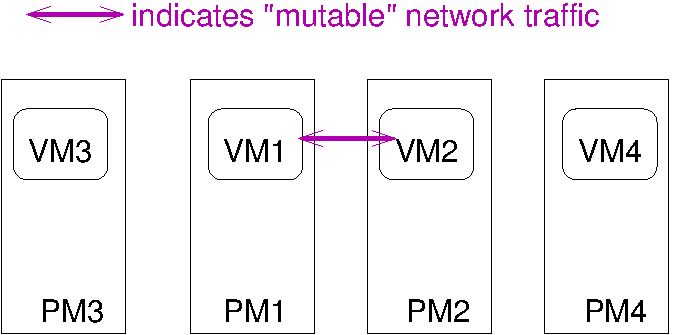
\includegraphics[scale=0.6]{figures/mutable-setup.pdf}
    \caption{Setup for \textit{mutable} network traffic generation: \textit{VM1 and VM2 communicate with each other, and get dispersed or colocated}}
    \label{fig:mutable-setup}
    \end{minipage}
    \hfill
    \begin{minipage}{0.45\textwidth}
    \centering
    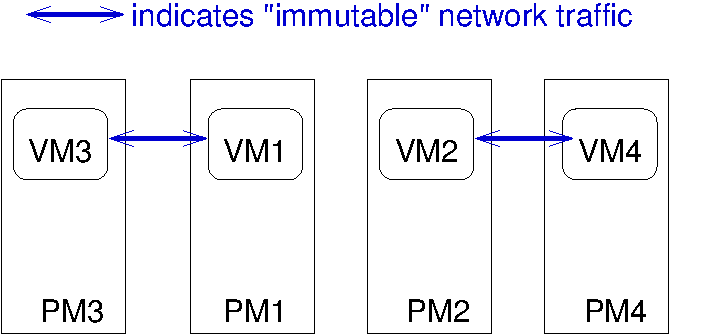
\includegraphics[scale=0.6]{figures/immutable-setup.pdf}
    \caption{Setup for \textit{immutable} network traffic generation: \textit{VM1 and VM2 have communication with other VMs (i.e., not with each other), and get dispersed or colocated}}
    \label{fig:immutable-setup}
    \end{minipage}
\end{figure}

Our experimental setup consisted of 4 VMs hosted on 4 PMs.
Fig.~\ref{fig:mutable-setup} shows the setup used to generate
mutable network traffic, and in contrast Fig.~\ref{fig:immutable-setup}
shows the setup for immutable network traffic experiment.
Here, the resource usage profiling is being performed
on VM1 and VM2 by placing them on dispersed and colocated
configurations, while the other two VMs are stationary.
Hence, the difference between these two setups is that 
mutable network traffic is generated between the pair VM1 and VM2,
whereas immutable network traffic is between two pairs,
(i)~VM1 and VM3, (ii)~VM2 and VM4.
Note that, in case of mutable traffic setup, colocation of
VM1 and VM2 (on PM1 or PM2) changes the nature of network traffic from 
\textit{inter-PM} to \textit{intra-PM}.
On the other hand, in case of immutable traffic setup, colocation or 
dispersion (on PM1 and PM2)
of VM1 and VM2 causes no change in the nature of their
network communication with VM3 and VM4, respectively\textemdash{}it stays
\textit{inter-PM} in both cases.

Note that, above we have assumed that colocation can happen only on 
PM1 or PM2, and not on PM3 or PM4. This is because of two main reasons.
Firstly, the above description is with respect to the VM pair of VM1 
and VM2. Secondly, if a single VM migration can cause it to be
colocated with multiple VMs or to be dispersed from one VM and
colocated with another, these scenarios are considered multi-VM
scenarios, and are handled separately as discussed in Section~\ref{sec:multi-vm}.

\section{Tool setup}
Every experiment is automated\textemdash{}simply specifying the IP addresses of the VMs and PMs,
specifying whether they need to be colocated or dispersed, 
and specifying load to be generated, is sufficient. The scripts
on \textit{controller} machine take these inputs and setup the experiment scenario
accordingly\textemdash{}VMs are instantiated on corresponding PMs (if they are not already running)
and the systems prepped for load generation. For example, disk read workload requires
the pre-creation of large dataset of size twice that of RAM. Additionally, \texttt{iptables}
rules are setup to capture the mutable and/or immutable network traffic being generated
in the given setup.

For each benchmark load, we start load generation on the two VMs and then start off the
logging on all concerned systems (the VMs and corresponding PMs). The metrics logging
is done every second, and continues for a minute. After a minute, logging is shut down and then
the load generation is stopped. The generated logs are then transferred to the log 
repository, for further analysis and model generation. 

For resource usage measurements, tools like \texttt{Xentop}, \texttt{top},
\texttt{sar} and \texttt{iptables} are used. We need the measurements along-with
timestamp information, so that different measurements can be correlated with
each other. Tools like \texttt{sar} and \texttt{top} report timestamps themselves,
however, \texttt{Xentop} does not provide timestamp information. Hence, we use
a perl-based wrapper for \texttt{Xentop}\textemdash{}the wrapper invokes \texttt{Xentop}
in batch mode every second, and notes the timestamp along-with Xentop output.

\section{Tool usage}
The main load generation tool in our \texttt{LoadGen} toolkit, 
is a C program \texttt{generate\_loads}. Its usage snippet is presented 
in Listing~\ref{lst:loadgen-usage}.

\lstset{language=C,
    caption={Listing of generate\_loads usage},
    label=lst:loadgen-usage
}
\begin{snippet}
Usage: ./generate_loads <daemonize> <expt-duration> [[<thread-type> <rate> <number> <name>]]

<expt-duration> should be integer
<thread-type> can be R, W, N, C
<rate> in Kbps for net with 1Mbps=1000Kbps and max=100Mbps & <rate> in perc for cpu
<number> can be 'number of 4k blocks' for R/W, 'number of 4kB' for N and xxxx for C
<name> can be file-prefix for R/W, web-server IP for N and xxxx for C
\end{snippet}

The 4-tuple [[<thread-type> <rate> <number> <name>]] seen in Listing~\ref{lst:loadgen-usage}
indicates the input per workload-type to be generated. Multiple such tuples can be input
on the command-line to indicate a mixed workload, as well. The different types of workloads
are indicated using the <thread-type> option\textemdash{}'R' for disk read, 'W' for disk write, 
'N' for network and 'C' for cpu workload. 
